%%%--------------------------------%%%
%%% Domain
%%%--------------------------------%%%
\newpage
\section{Software Specification}
\label{sec:domainB}

\subsection{Purpose and Scope}
\label{sec:domainBa}
There are risk management tools on the market to support project managers in their risk management activities. Some tools have a similar focus to this work \cite{OperationalRiskManagement}, \cite{RiskManagementSoftware} others are oriented towards company risk managment \cite{QHSERiskCompliance} wheareas again others are project management tools with a risk managment section \cite{https://www.ntaskmanager.com/}. Those programs contain similar features as discussed in \ref{sec:theorieAc} and \ref{sec:theorieAc}. They do not cover user engagement however. To prevent negligence in the course of project life we want to add gamification elements as discussed in \ref{sec:TBD} to incorporate not only process support but to also consider the human factor.
We want to develop a flexible application prototype to support project managers and their teams with their risk management activities. The app should cover all four phases of the risk management process, it should be able to learn with the teams’ experiences and it should be engaging.
We do not want to provide pre-defined risks or mitigations in the scope of this work. We also explicitly focus on project risk management, not on company risk management or IT security issues. 

\subsection{Functionalities}
\label{sec:domainBb}
We have developed eleven use cases that describe the program functionalities. There are basic functionalities which cover the user and project administration. Risk management related functionalities cover the administration and evaluation of risks and risk responses. The learning aspect is covered by what we call a ‘risk pool’ and finally there are gamification use cases for user engagement. The detailed descriptions of these functionalities are subject of the following sections. 

\subsubsection{Overall Use Case Diagram}
\label{sec:domainBba}
\begin{figure}[H]
	\centering
	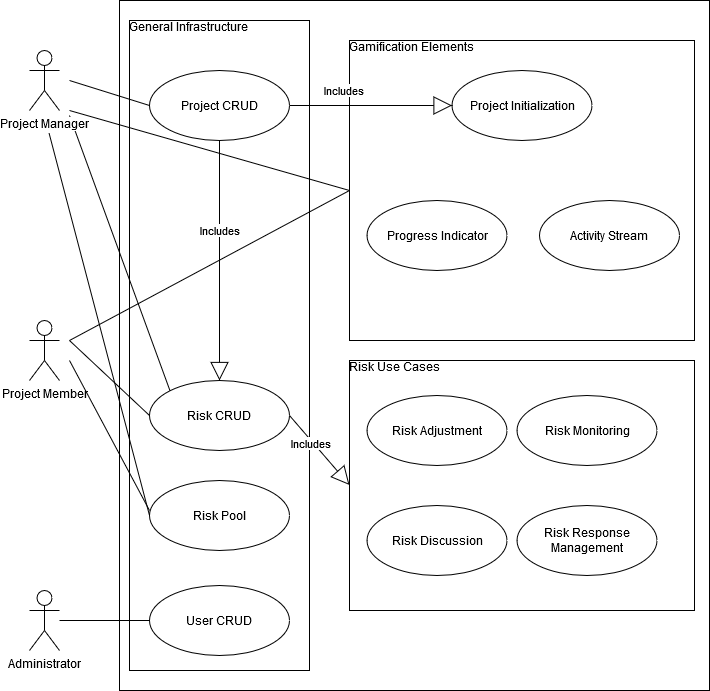
\includegraphics[width=1.0\textwidth]{Content/Domain/OUCD.png}
	\caption{Overall Use Case Diagram}
	\label{fig:label10}
\end{figure}

\spacing{1}
%%%--------------------------------%%%
%%% Use Cases N
%%%--------------------------------%%%
\foreach \i in {01,02,03,04,05,06,07,08,09,10,...,99} {%
	\edef\FileName{Content/Domain/UC/\i_uc}%
	\IfFileExists{\FileName}{%
		\input{\FileName}
	}
	{%
		% File does not exist
		
	}
}%foreach
\spacing{1.5}


\subsection{Requirements}
\label{sec:domainBc}
This project is being developed as a student research project and part of the authors’ curriculum and thus subject to the regulations of the Duale Hochschule Baden-Württemberg \cite{ leitlinienfachkommissiontechnikLeitlinienFurBearbeitung}. Given the limitations due to this circumstance we still aspire for our software to meet the following requirements.
\paragraph*{Usability}
\label{sec:domainBca}
For the application to be usable on desktop and mobile device we use responsive design. We also aim for intuitive design using known symbols and functionalities to ensure user comfort. We adhere to design guidelines and we used a mock-up prototype to receive early user feedback.
\paragraph*{Reliability}
\label{sec:domainBcb}
We do not intend to provide hosting for the software. As project health is sensitive information for a company so this data is best left under the repective company's control. Therefore in terms of reliabilty we aim to provide a stable software but have no further service level agreements. To ensure software stability we make use of state of the art technology such as React with Redux, Spring Boot and a Postgre SQL database.
\paragraph*{Performance}
\label{sec:domainBcc}
To make our application fast and scalable we use RESTful apis. Our front end is designed as a single page application for faster in-app performance. For future development this also offers the option to develop offline functionalities. Our back end uses a container based approach using docker and docker compose.
\paragraph*{Supportability}
\label{sec:domainBcd}
We use sonar to ensure code quality for future maintance and expandability. We work with contious integration, deployment and delivery to maintain program stability using appropiate unit and integration tests. Furthermore we do code reviews and follow the SOLID design principles.  

\subsection{Design Constraints}
\label{sec:domainBd}
The software is designed as a web application so internet access will be required. As a PWA the application can support offline functionality however that will not be implemented within the scope of this project. Due to the chosen technology we also cannot guarantee all features to be available for every webbrowser, howver the application is designed to provide the core functionalities even without additional PWA features.


\subsection{Interfaces}
\label{sec:domainBe}

\subsubsection{User Interfaces}
\label{sec:domainBea}
The application will start on the home screen. After registration and login the home screen will transform into the specific user's activity stream page which covers all recent events relevant to the user. From there the user can navigate to their project screen which lists all their project. The project detail view also covers the risks for the respective project. The risk detail view incorporates risk responses.
When adding new risks users can open the risk pool to view all pool risks available to the company.
\subsubsection{Further Interfaces}
\label{sec:domainBeb}
Since our PWA is supposed to be re-engaging we use push notification to enhance user commitment. To do so we use Google's Firebase Cloud Messaging. Documentation for Firebase can be found at \href{https://firebase.google.com/docs/cloud-messaging}{https://firebase.google.com/docs/cloud-messaging}.
